\documentclass[12pt,italian]{article}
\usepackage[italian]{babel}
\usepackage[a4paper, margin=2cm]{geometry}
\usepackage{graphicx}
\graphicspath{{./images/}}
\usepackage{subfig}
\usepackage{amsmath}
\usepackage{circuitikz}
\usepackage{caption}
\usepackage{cleveref}
\usepackage{amsfonts}

\usepackage{tikz}
\usetikzlibrary{patterns,plotmarks}

\hyphenation{ELVIS}
\newcommand{\err}[1]{\textcolor{red}{#1}}

%\usepackage{fontspec} \setmainfont{calibri}
%\usepackage{titlesec}
%\titleformat{\section}
%{\normalfont\normalsize\itshape}{\thesection.}{1em}{}
%\titlespacing{\section}{0pt}{1em}{0pt}


\title{Misure di grandezze caratteristiche su un circuito crossover}
\author{Enrico Barbuio \\ 0001117553 \and Giacomo Cicala \\ 0001122965} 
\date{\err{data}}

\begin{document}
\maketitle
\section*{Abstract}
L'esperimento ha avuto come obiettivo la progettazione e la realizzazione, su
breadboard ELVIS II, di un crossover RLC a tre vie (woofer, midrange, tweeter),
corredato dallo studio analitico del comportamento in regime sinusoidale e dal
confronto con le misure sperimentali. Dal punto di vista qualitativo si è
osservato che la risposta in ampiezza del woofer decresce verso zero alle alte
frequenze, quella del tweeter cresce asintoticamente al valore del generatore e il
midrange presenta un picco alla risonanza; le misure di fase confermano
l'inversione di $ \pm 90^\circ $ (\err{FALSO}) fuori banda e la coerenza in
banda di taglio. Il valore teorico della frequenza di crossover tra woofer e
tweeter, calcolato dalla relazione analitica, è risultato

\begin{equation*}
	f_{c} = (10.40 \pm 0.12)  \text{ kHz}
\end{equation*}

\noindent
mentre la misura sperimentale ha fornito

\begin{equation*}
	f_{c} = (\cdots \pm \cdots) \text{ kHz}
\end{equation*}

\noindent
La frequenza di risonanza del midrange attesa è
\begin{equation*}
	f_{r} = (10.65 \pm 0.10)  \text{ kHz}
\end{equation*}

\noindent
e quella misurata
\begin{equation*}
	f_{r} = (\cdots \pm \cdots)  \text{ kHz}
\end{equation*}
\err{aggiungere anche differenza di fase al crossover?}

\section*{Introduzione}

L'esperimento svolto in laboratorio è incentrato sulla realizzazione di un
circuito RLC, sullo studio analitico del comportamento atteso e sul confroto di
questo con le misure effettuate. Il circuito scelto è un crossover a tre vie:
un circuito filtrante che divide un segnale su tre canali al fine di
ottimizzare la riproduzione sonora per tutta la gamma di frequenze. Nel canale
del woofer si trova un filtro passa-basso (RL serie), nel midrange un filtro
passa-banda (RLC serie) e infine nel tweeter un filtro passa-alto (RC serie).
Dalla legge di Ohm e dalle leggi di Kirchhoff simboliche per tensioni e
correnti, utilizzando il metodo dei fasori, è stata ricavata la soluzione
stazionaria della differenza di potenziale ai capi del generatore e ai capi
delle resistenze di woofer, medi e tweeter. Riportiamo qui le loro ampiezze

\begin{equation}
	\left| \mathbf{V_{g}}(\omega) \right| = \left| 1 - \frac{R_g}
	{\mathbb{Z}_{tot}(\omega)}\right| V_{0}
	\label{eq:Vg}
\end{equation}

\begin{equation}
	\left| \mathbf{V_{w}}(\omega) \right| = \left| \frac{R_{w}}
	{\mathbb{Z}_{w}(\omega)}\right|\left| \mathbf{V_{g}}(\omega) \right|
	\label{eq:Vw}
\end{equation}

\begin{equation}
	\left| \mathbf{V_{m}}(\omega) \right| = \left| \frac{R_{m}}
	{\mathbb{Z}_{m}(\omega)}\right|\left| \mathbf{V_{g}}(\omega) \right|
	\label{eq:Vm}
\end{equation}

\begin{equation}
	\left| \mathbf{V_{t}}(\omega) \right| = \left| \frac{R_{t}}
	{\mathbb{Z}_{t}(\omega)}\right|\left| \mathbf{V_{g}}(\omega) \right|
	\label{eq:Vt}
\end{equation}

\noindent
e le rispettive fasi (\err{decidere dove esplicitare e definire simboli, togli fase del generatore giustificando in appendice}) (\ref{sec:fasi})

\begin{equation}
	\phi_{g}(\omega) = Arg(\mathbf{V_{g}}(\omega))
\end{equation}

\begin{equation}
	\phi_{w}(\omega) = Arg(\mathbf{V_{g}}(\omega)) - Arg(\mathbb{Z}_{w}(\omega))
\end{equation}

\begin{equation}
	\phi_{m}(\omega) = Arg(\mathbf{V_{g}}(\omega)) - Arg(\mathbb{Z}_{m}(\omega))
\end{equation}

\begin{equation}
	\phi_{t}(\omega) =  Arg(\mathbf{V_{g}}(\omega)) - Arg(\mathbb{Z}_{t}(\omega))
\end{equation}
\\
tutto in funzione della pulsazione.

Per quanto riguarda le ampiezze delle tensioni in funzione della frequenza ci
aspettiamo che: il woofer abbia un massimo a basse frequenze e un andamento
decrescente asintoticamente a zero per le alte, il tweeter tenda
asintoticamente al generatore, mentre il midrange dovrà avere un picco alla
frequenza di risonanza. Invece, per quanto riguarda le fasi, woofer e tweeter
dovrebbero essere in fase con il generatore rispettivamente a basse e alte
frequenze, mentre saranno in ritardo e in anticipo di fase di $90^\circ$ nel
caso contrario. Il midrange dovrà essere in fase con il generatore alla
frequenza di risonanza.

Imponendo l'uguaglianza tra le relazioni \eqref{eq:Vw} e \eqref{eq:Vt} è
possibile ricavare il valore atteso della frequenza di crossover \eqref{eq:fc},
cioè la frequenza alla quale il woofer e il tweeter hanno la tensione di
ampiezza uguale.

\begin{equation}
	f_{c} = \frac{1}{2\pi}\sqrt{\frac{\sqrt{4 (R_{w} R_{t} L_{w})^2 + C_{t}^2(2
				R_{w} R_{Lw} R_{t}^2 + (R_{Lw} R_{t})^2)^2}}{2 C _{t} (L_{w} R_{t})^2 } -
		\frac{R_{w} R_{Lw}}{L_{w}^2} - \frac{R_{Lw}^2}{2 L_{w}^2}}
	\label{eq:fc}
\end{equation}

\noindent
Inoltre, da \eqref{eq:Vm} è possibile calcolare la frequenza di risonanza attesa del midrange \eqref{eq:fr} (vedi \cref{sec:resFreq}).

\begin{equation}
	f_{r} = \frac{1}{2\pi}\sqrt{\frac{1}{L_{m} C_{m}}}  %equazione approssimata
	\label{eq:fr}
\end{equation}

\noindent
Infine, si può ottenere \err{la differenza di fase tra tweeter e woofer alla frequenza di crossover}.

\begin{equation}
	booh non so se farlo
\end{equation}

\section*{Apparato sperimentale e svolgimento}

Il circuito (fig. \ref{fig:schema_elettrico}) è stato realizzato su una
breadboard. La scheda NI ELVIS II (\cref{fig:Elvis}) è stata utilizzata come
dispositivo DAQ unitamente ad un computer dotato di software apposito
all'acquisizione e all'elaborazione delle misure. Per l'analisi in frequenza di
ampiezza e fase è stato acquisito ciascun canale separatamente, con sweep
ripetuti. In ogni prova l'analog input \texttt{A1} è stato collegato al canale
di interesse mentre il canale \texttt{A0} è rimasto collegato al generatore di
tensione, utilizzandolo come trigger e riferimento per la fase. Come range di
frequenze è stato scelto: $1$ kHz - $50$ kHz; questo per evidenziare il punto
di crossover ma anche per vedere l'andamento a basse e alte frequenze. Al fine
di massimizzare la frequenza di campionamento, le tensioni sono state misurate
in modalità referenced single ended collegando a massa il ramo in comune alle
resistenze. Ciò ha permesso un campionamento a $500$ kHz per canale, con $2000$
sample per ciascuna acquisizione, abbastanza per includere $4$ o più periodi a
qualsiasi frequenza del range.

I componenti del circuito sono stati misurati tramite il multimetro di ELVIS
II, i loro valori e le rispettive incertezze (strumentali) si trovano in
\cref{tab:componenti} (\err{mettere la tabella nei risultati?}).

\noindent
\begin{minipage}[b]{0.6\textwidth}
	\vspace{0pt}
	\centering
	\begin{circuitikz}[scale=1]
		% generatore
		\draw (8,0) --
		(0,0) --
		(0,1.5) to[sinusoidal voltage source]
		(0,3) to[R, l=$R_g$, color=blue, bipoles/resistor/height=0.15, bipoles/resistor/width=0.5]
		(0,4) --
		(0,5.5) --
		(8,5.5);

		\draw(-0,4.5) to[short, -o]
		(-0.6,4.5) node[left]{$v_g$};
		\draw (-0,1) -- (-0.6,1) node[ground]{};

		% woofer
		\draw (3,5.5) --
		(3,4.5) to[L=$L_w$]
		(3,3.5) to[R, l=$R_{Lw}$, color=blue, bipoles/resistor/height=0.15, bipoles/resistor/width=0.5]
		(3,2.5) --
		(3,2) to[R=$R_w$] (3,0);
		\draw (3,2) to [short, -o] (3.5, 2) node[right]{$v_w$};

		% mid
		\draw (5.5,5.5) to [C=$C_m$]
		(5.5,4.25) to [L=$L_m$]
		(5.5,3.25) to [R, l=$R_{Lm}$, color=blue, bipoles/resistor/height=0.15, bipoles/resistor/width=0.5]
		(5.5,2.25) --
		(5.5,2) to[R=$R_m$] (5.5,0);

		\draw (5.5,2) to [short, -o] (6, 2) node[right]{$v_m$};

		%tweeter
		\draw (8,5.5) to[C=$C_t$]
		(8,2) to[R=$R_t$] (8,0);

		\draw (8,2) to
		[short, -o] (8.5, 2) node[right]{$v_t$};
	\end{circuitikz}
	\captionof{figure}{Schema elettrico del circuito. I punti $v_g, v_w, v_m,
			v_t$ sono stati collegati agli analog input di ELVIS II per le relative
		misure di tensione. I pedici $g$, $w$, $m$, $t$ indicano i rami del generatore, woofer,
		midrange e tweeter. I componenti non ideali sono disegnati in blu.}\label{fig:schema_elettrico}
\end{minipage}
\begin{minipage}[b]{0.4\textwidth}
	\vspace{0pt}
	\centering
	\begin{alignat*}{2}
		 & R_w    &  & =(3293 \pm 2) \text{ \Omega}      \\
		 & L_w    &  & =(47.2 \pm 0.5) \text{ mH}        \\
		 & R_{Lw} &  & =(120.00 \pm 0.15) \text{ \Omega} \\[1em]
		 & R_m    &  & =(3287 \pm 2) \text{ \Omega}      \\
		 & L_m    &  & =(46.8 \pm 0.5) \text{ mH}        \\
		 & R_{Lm} &  & =(120.70 \pm 0.15) \text{ \Omega} \\
		 & C_m    &  & =(4.76 \pm 0.05) \text{ nF}       \\[1em]
		 & R_t    &  & =(3295 \pm 2) \text{ \Omega}      \\
		 & C_t    &  & =(4.76 \pm 0.05) \text{ nF}       \\[1em]
		 & R_g    &  & =50 \text{ \Omega \ (dichiarata)}
	\end{alignat*}
	\captionof{table}{Valori componenti.}
	\label{tab:componenti}
\end{minipage}

\begin{figure}[h]
	\centering
	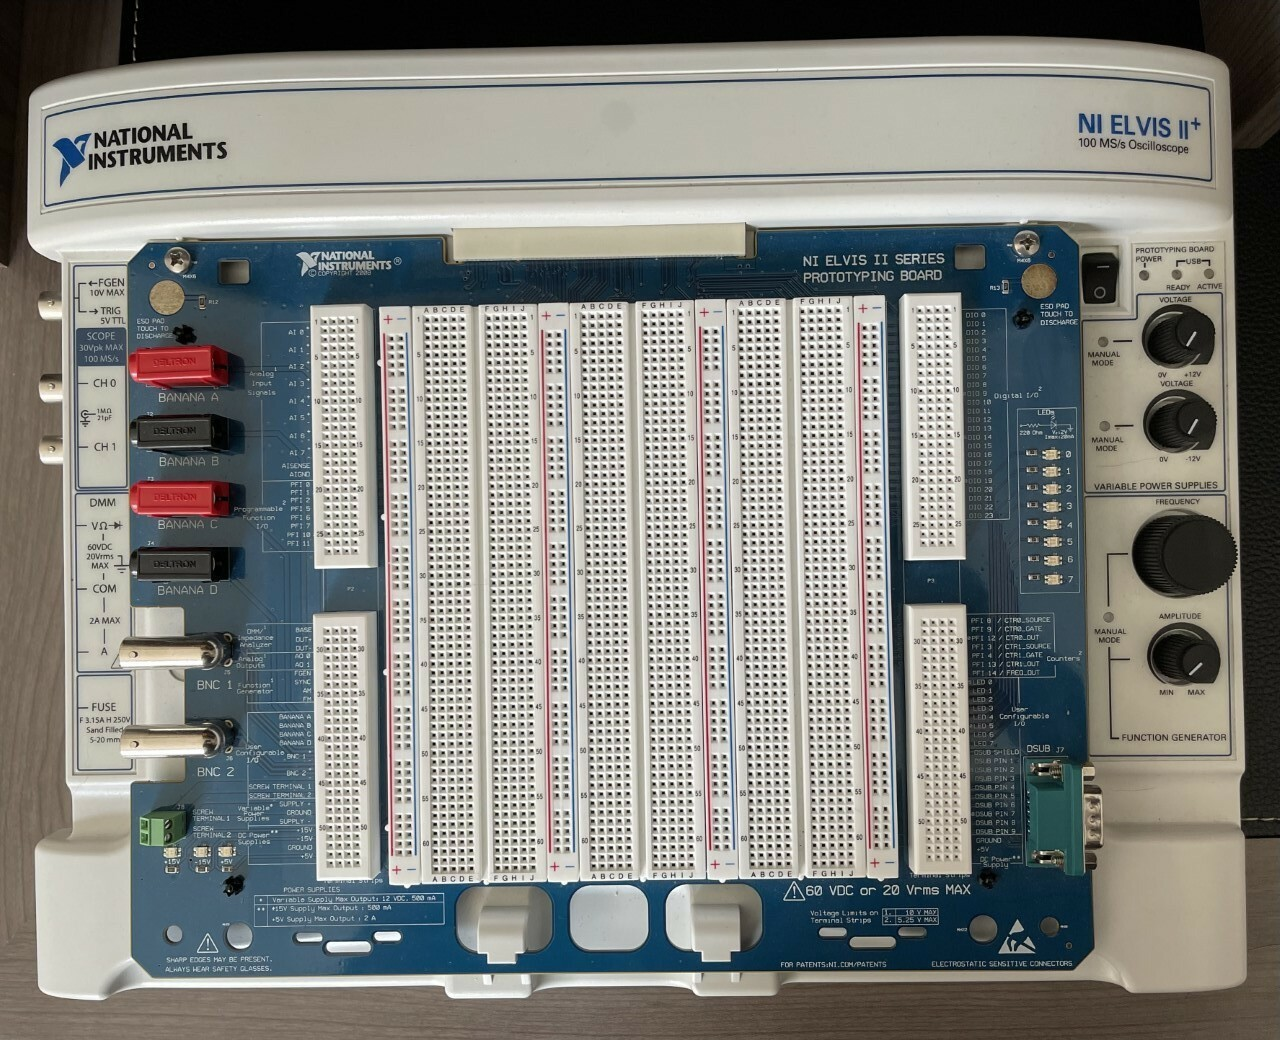
\includegraphics[width=0.5\textwidth]{Elvis.jpg}
	\caption{Foto della scheda NI ELVIS II (\err{sistema foto (c'è anche foto circuito)})}
	\label{fig:Elvis}
\end{figure}

\section*{Risultati e discussione}
Dalle misure delle componenti riportate in \cref{tab:componenti} e
dall'equazione \eqref{eq:fc} abbiamo ricavato la miglior stima del valore
atteso della frequenza di crossover:

\begin{equation*}
	f_{c} = (10.40 \pm 0.12)\  \text{ kHz} \hspace{2cm} \frac{\Delta f_{c}}{f_{c}} = 1.2 \ \%
\end{equation*}

\noindent
Analogamente, la frequenza di risonanza del midrange attesa è risultata:

\begin{equation*}
	f_{r} = (10.65 \pm 0.10)\  \text{ kHz} \hspace{2cm} \frac{\Delta f_{r}}{f_{r}} = 1 \ \%
\end{equation*}
Questo valore fa fede alla relazione ideale Eq.~\eqref{eq:fr} perché gli effetti del circuito reale sono risultati inferiori
all'errore strumentale, più dettagli in \cref{sec:resFreq}. Entrambe le incertezze sono state propagate linearmente e sono da considerarsi assolute.

Per ricavare $f_{c}$ e $f_{r}$ dalle misure di ampiezza, si sono eseguiti dei
fit in un intorno ristretto delle due frequenze interessate ($ 7 $ kHz - $ 14 $
kHz) con le funzioni (\ref{eq:Vg}), (\ref{eq:Vw}), (\ref{eq:Vm}) e
(\ref{eq:Vt}) (\cref{fig:amp_sweep}). Le incertezze associate ai punti
sperimentali risultano

\begin{equation*}
	\Delta V = 1.9 \text{ mV} \hspace{2cm} \Delta f = 0.186 \text{ Hz}
\end{equation*}

\noindent
e sono entrambi errori di risoluzione strumentale presi dal datasheet di ELVIS
II.

\begin{figure}[h]
	\centering
	\includegraphics[width=0.5\textwidth]{example-image}
	\caption{Grafico delle ampiezze delle tensioni in funzione della frequenza per il woofer, midrange, tweeter e generatore. I fit sono eseguiti nel range $7$ kHz - $14$ kHz e le funzioni risultanti disegnate su tutto il range di acquisizione.}\label{fig:fc_fr}
	\label{fig:amp_sweep}
\end{figure}

Uguagliando le funzioni risultanti del woofer e del tweeter, si è calcolata
numericamente $f_{c}$, allo stesso modo $f_{r}$ è stata calcolata numericamente
come frequenza corrispondente al massimo della funzione di fit. Le incertezze
sono state propagate in quadratura e vanno considerate come statistiche.
Riportiamo di seguito le stime ottenute e le loro incertezze:

\begin{equation*}
	f_{c} = (10.64 \pm 0.02) \text{ kHz}
\end{equation*}
\begin{equation*}
	f_{r} = (10.89 \pm 0.16)\  \text{ kHz}
\end{equation*}

Per verificare le proprietà filtranti del circuito è possibile svolgere
un'analisi qualitativa delle ampiezze per il range di frequenze complessivo
acquisito: dalla (\cref{fig:fc_fr}) si può notare, come ci aspettavamo, che
woofer, midrange e tweeter si comportano rispettivamente come un filtro
passa-basso, un passa-banda e un passa-alto; tuttavia si osserva che il modello
da noi utilizzato non si adatta ai dati sperimentali per range di frequenze
così ampi.

Il grafico nelle fasi si è discostato parecchio dalla funzione attesa. Data la
complessità del modello non siamo riusciti a ottenere un fit convergente
neanche su regioni ristrette, di conseguenza non abbiamo potuto associare un
incertezza significativa alle misure ricavate in questo modo.

\begin{equation*}
	f_{c} = 10.601 \text{ kHz} \hspace{2cm} f_{r} = 10.791 \text{ kHz}
\end{equation*}

Si è deciso allora di approssimare localmente (nell'intervallo $10$ kHz -
$11.2$ kHz) il grafico delle fasi con una retta (fig.). In questo modo abbiamo
misurato:

\begin{equation*}
	f_{c} = (10.60 \pm 0.03)\  \text{ kHz} \hspace{2cm}	f_{r} = (10.797 \pm 0.008)\  \text{ kHz}
\end{equation*}

\begin{figure}[h]
	\centering
	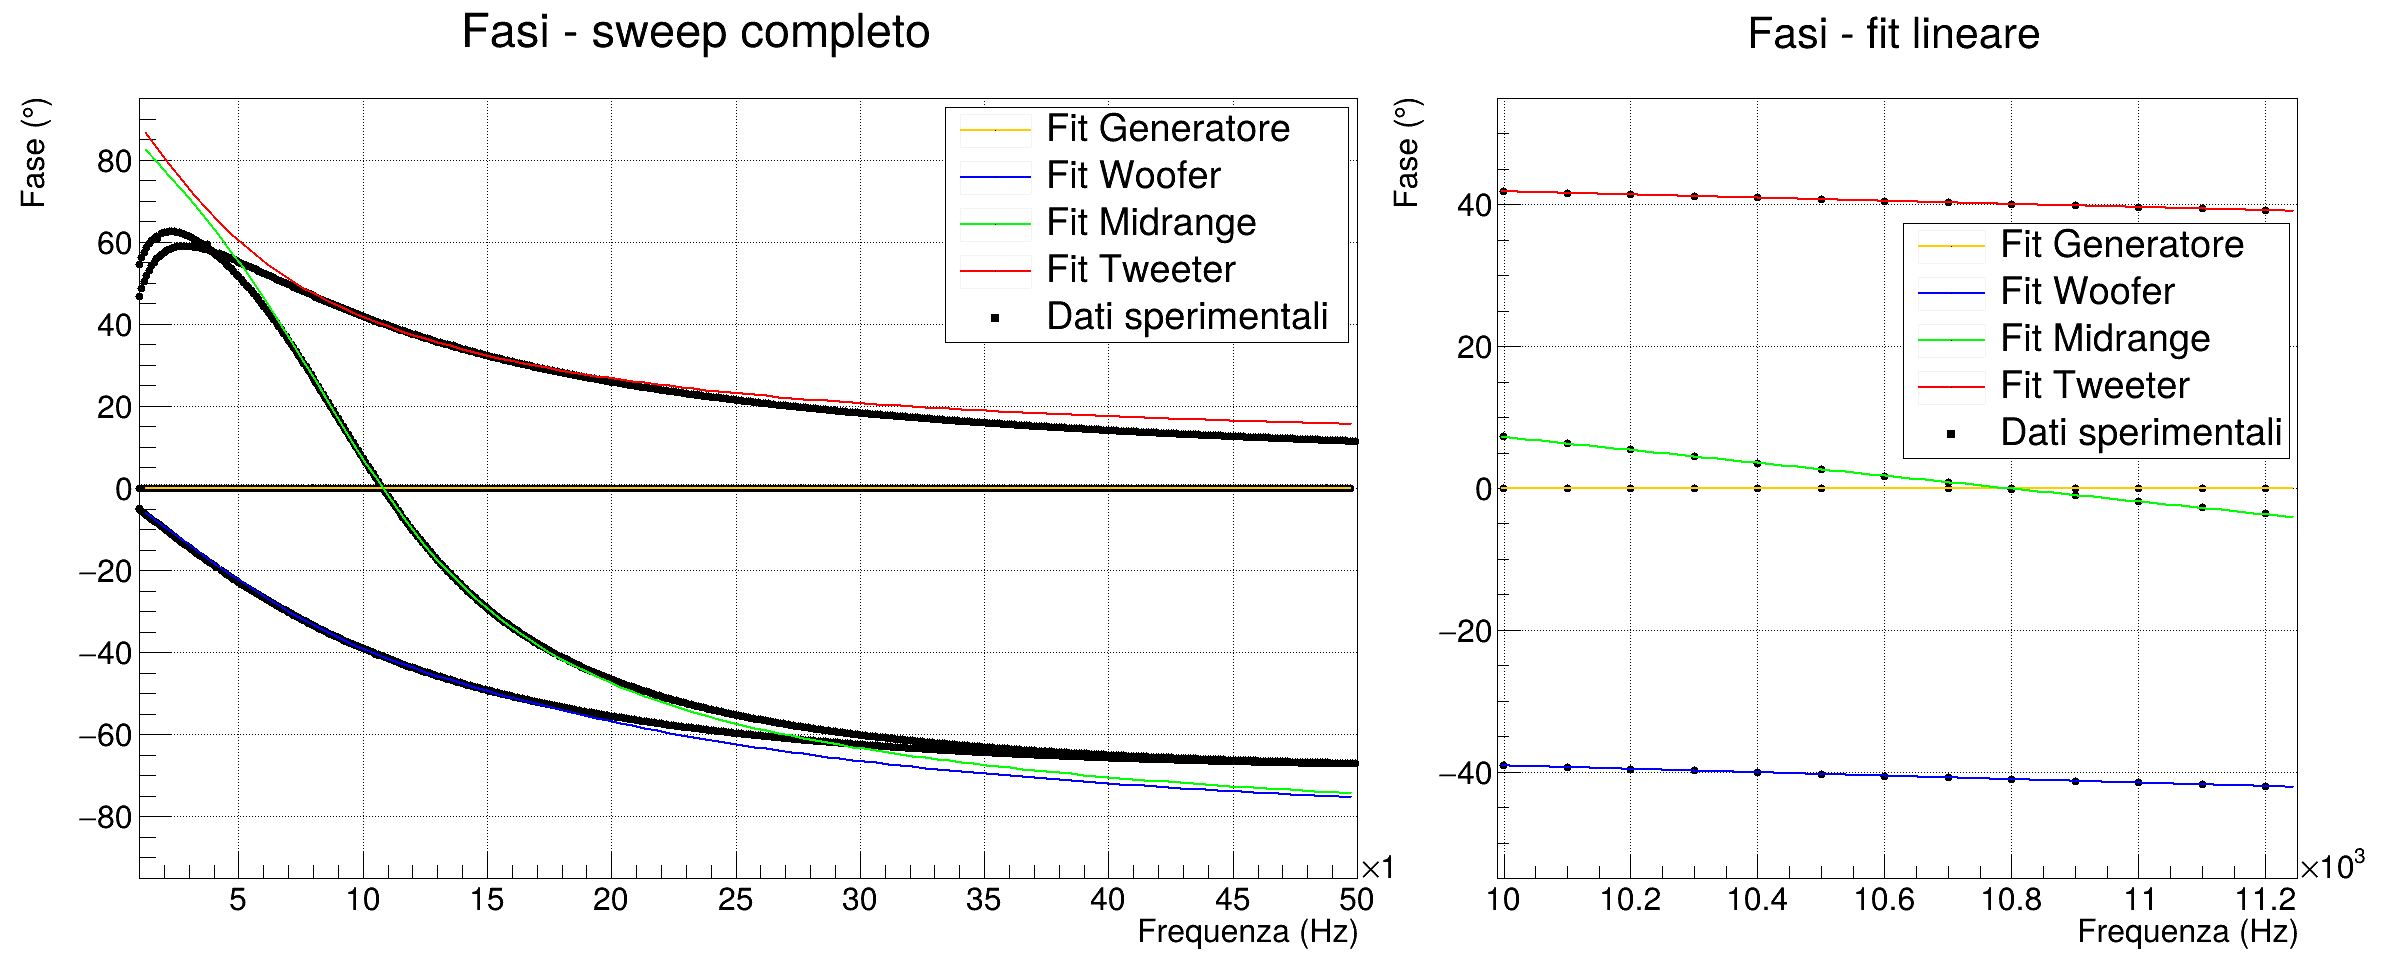
\includegraphics[width=\textwidth]{fig_fase.png}
	\caption{A sinistra: grafico delle fasi in funzione della frequenza per il woofer
		(blu), il midrange (verde), il tweeter (arancione) e per il generatore (rosso);
		fit ristretto al range $8$ kHz - $16$ kHz. A destra: fit lineare degli stessi dati da $10$ kHz a $11.2$ kHz.}\label{fig:phase_sweep}
\end{figure}

\section*{Conclusioni}

\appendix
\section{Appendici}
\subsection{Tensioni ai capi delle resistenze}
\label{sec:tensioni}

\begin{equation*}
	\mathbb{Z}_{load}(\omega) = \left(\frac{1}{\mathbb{Z}_{w}(\omega)} + \frac{1}{\mathbb{Z}_{m}(\omega)} + \frac{1}{\mathbb{Z}_{t}(\omega)}\right)^{-1}
\end{equation*}

\begin{equation}
	\left| \mathbf{V_{g}}(\omega) \right| = \left| \frac{\mathbb{Z}_{load}(\omega)}
	{R_{g}+\mathbb{Z}_{load}(\omega)}\right| \mathbf{V}
\end{equation}

\begin{equation}
	\left| \mathbf{V_{w}}(\omega) \right| = \left| \frac{R_{w}}
	{\mathbb{Z}_{w}(\omega)}\right|\left| \mathbf{V_{g}}(\omega) \right| = \left| \frac{R_{w}}
	{R_{w}+R_{Lw} + j \omega L_w}\right|\left| \mathbf{V_{g}}(\omega) \right|
\end{equation}

\begin{equation}
	\left| \mathbf{V_{m}}(\omega) \right| = \left| \frac{R_{m}}
	{\mathbb{Z}_{m}(\omega)}\right|\left| \mathbf{V_{g}}(\omega) \right| = \left| \frac{R_{m}}{R_{m}+R_{Lm} + j (\omega L_m - \frac{1}{\omega C_{m}})} \right| \left| \mathbf{V_{g}}(\omega) \right|
\end{equation}

\begin{equation}
	\left| \mathbf{V_{t}}(\omega) \right| = \left| \frac{R_{t}}
	{\mathbb{Z}_{t}(\omega)}\right|\left| \mathbf{V_{g}}(\omega) \right| = \left| \frac{R_{t}}{R_{t} + j (-\frac{1}{\omega C_{t}})}\right|\left| \mathbf{V_{g}}(\omega) \right|
\end{equation}

\subsection{Fasi delle tensioni}
\label{sec:fasi}

\begin{equation}
	\phi_{w}(\omega) = - \arctan\left(\frac{\omega L_{w}}{R_{w}+R_{Lws}}\right)
\end{equation}

\begin{equation}
	\phi_{m}(\omega) = - \arctan\left(\frac{\omega L_{m} - \frac{1}{\omega C_{m}}}{R_{m}+R_{Lm}}\right)
\end{equation}

\begin{equation}
	\phi_{t}(\omega) = \arctan\left(\frac{1}{\omega R_{t} C_{t}}\right)
\end{equation}

\subsection{Frequenza di risonanza}\label{sec:resFreq}
La prima misura è data dalla relazione ideale Eq. \eqref{eq:fr}; la seconda
tiene conto anche degli effetti non ideali ed è stata ricavata numericamente
come frequenza corrispondente al massimo di Eq. \eqref{eq:Vm}.

\begin{equation*}
	f_{r}^{\text{(ideale)}} = 10652 \text{ Hz} \hspace{2cm} f_{r}^{\text{(reale)}} = 10651 \text{ Hz}
\end{equation*}
% f_r
Poichè l'errore percentuale che si commette prendendo $f_{r}^{\text{(ideale)}}$
come miglior stima è solamente $\varepsilon_{f_r} \approx 0.01\%$, si è scelto
di utilizzare questa stima per poter propagare con semplicità l'incertezza, che
risulta essere

\begin{equation*}
	\begin{alignedat}{2}
		\frac{\Delta f_{r}}{f_{r}} = & \frac{1}{2} \frac{\Delta L_{m}}{L_{m}} &  & + \frac{1}{2} \frac{\Delta C_{m}}{C_{m}} \\
		=                            & 0.005                                  &  & + 0.005
		= 0.01 = 1 \ \%
	\end{alignedat}
\end{equation*}
ossia due ordini di grandezza più grande di $\varepsilon_{f_r}$

\subsection{Incertezze}

\noindent
\err{TOGLIERE QUESTO PARAGRAFO?}
mentre per la miglior stima sulla sua incertezza abbiamo propagato linearmente
le incertezze strumentali dovute alla misura dei componenti (\err{sistema cifre dec})

\begin{equation*}
	\begin{alignedat}{5}
		\Delta f_{c} = & \left|\frac{\partial f_{c}}{\partial R_{w}}\right| \Delta R_{w} &  & +  \left|\frac{\partial f_{c}}{\partial R_{Lw}}\right| \Delta R_{Lw} &  & + \left|\frac{\partial f_{c}}{\partial L_{w}}\right| \Delta L_{w} &  & + \left|\frac{\partial f_{c}}{\partial R_{t}}\right| \Delta R_{t} &  & + \left|\frac{\partial f_{c}}{\partial C_{t}}\right| \Delta C_{t} \\
		=              & ( 3.16                                                          &  & +  0.269                                                             &  & + \colorbox{yellow}{52.9}                                         &  & + 3.28                                                            &  & + \colorbox{yellow}{56.9} ) \text{ Hz}                            \\
		=              & 117 \text{ Hz}
	\end{alignedat}
\end{equation*}

\noindent
dove sono stati evidenziati i termini più significativi.
\end{document}